\documentclass[11pt,a4paper]{report}

\usepackage[a4paper, margin=1in]{geometry}
\usepackage{polski}
\usepackage[utf8]{inputenc}
\usepackage{indentfirst}
\usepackage{hyperref}
\usepackage{tikz}

\usetikzlibrary{positioning}
\usetikzlibrary{calc}

\def\console #1{\begingroup\fontfamily{qcr}\selectfont#1\endgroup}
\newenvironment{multiconsole}{\begingroup\fontfamily{qcr}\selectfont}{\endgroup}

\title{\Huge GridGraph - Dokumentacja}
\author{Skoczek Mateusz, Jędrzejewski Sebastian}
\date{\today}



\begin{document}
    \maketitle
        




    \begin{abstract}
        Dokument zawiera specyfikację funkcjonalną i implementacyjną dotyczącą projektu \textsl{GridGraph} oraz opis testów programu.
    \end{abstract}





    \tableofcontents
    \thispagestyle{empty}





    \newpage
    \chapter{Specyfikacja funkcjonalna}




    \newpage
    \section{Cel projektu}

    Program \console{GridGraph} ma na celu wygenerowanie oraz zapis do pliku (lub na standardowe wyjście) grafu siatkowego o podanych paramentrach lub wczytanie grafu z pliku (lub ze standardowego wejścia) i sprawdzenie wybranych jego parametrów. Program działa w trybie wsadowym. Grafy są przedstawiane w plikach w postaci listy sąsiedztwa.



    \newpage
    \section{Opis funkcji}
    Program może działać w dwóch trybach: zapisu (\console{write}) i czytania (\console{read}).

    \vspace{2em}

    W trybie zapisu program generuje graf o określonej przez użytkownika szerokości (ilości kolumn) (\console{width}), wysokości (ilości wierszy) (\console{height}), minimalnej (\console{edge\_weight\_min}) i maksymalnej (\console{edge\_weight\_max}) wagi krawędzi oraz minimalnej (\console{edge\_count\_min}) i maksymalnej (\console{edge\_count\_max}) ilości krawędzi wychodzących z jednego wierzchołka, a następnie zapisuje go w formie listy sąsiedztwa do pliku określonego przez użytkownika (lub wypisuje na standardowe wyjście).

    Jeżeli graf zostanie pomyślnie zapisany do pliku (lub wypisany na standardowe wyjście), program zwróci \console{0}. W przeciwnym wypadku zostanie wyświetlony komunikat błędu, a program zwróci \console{1}.
    
    \vspace{2em}

    W trybie czytania program wczytuje graf zapisany (w formie listy sąsiedztwa) w określonym przez użytkownika pliku (lub czyta ze standardowego wejścia), a następnie sprawdza określone przez użytkownika właściwości grafu:
    \begin{itemize}
        \item Spójność grafu (\console{connectivity})
        \item Najkrótsza ścieżka z węzła A do innych węzłów (\console{shortest\_path\_a}) lub do określonego węzła B (\console{shortest\_path\_a} oraz \console{shortest\_path\_b})
    \end{itemize}

    Jeżeli graf został wczytany oraz sprawdzony pomyślnie, zostanie wyświetlony wynik sprawdzania, a następnie program zwróci \console{0}. W przeciwnym wypadku zostanie wyświetlony komunikat błędu, a program zwróci \console{1}

    \vspace{1em}

    Przykład (graf spójny, ścieżka istnieje):


    \begin{multiconsole}
        \noindent
        Connectivity: connected

        \noindent
        Shortest path from 0 to 10 (weight): 0-3-4-6-9-10 (0.778)
    \end{multiconsole}

    \vspace{1em}

    Przykład (graf niespójny, ścieżka nie istnieje):

    \begin{multiconsole}
        \noindent
        Connectivity: disconnected

        \noindent
        Shortest path from 0 to 10 (weight): path does not exist
    \end{multiconsole}



    \newpage
    \section{Opis wywołania}

    Jeżeli nie zostanie wybrany tryb (tzn. nie zostanie przekazany argument \console{--write/-w} lub \console{--read/-r}) zostanie wyświetlona pomoc.

    \subsection{Tryb zapisu}

    \textbf{Wywołanie:}
    \console{./gridgraph --write/-w [argumenty]}

    \vspace{1em}

    \textbf{Argumenty:}

    \begin{itemize}
        \item \console{--width/-xw} (Szerokość grafu - liczba kolumn)
        \begin{description}
            \item[Typ:] Liczba naturalna
            \item[Zakres:] $>$ 0 
            \item[Wymagany:] TAK
        \end{description}
        \item \console{--height/-xh} (Wysokość grafu - liczba wierszy)
        \begin{description}
            \item[Typ:] Liczba naturalna
            \item[Zakres:] $>$ 0 
            \item[Wymagany:] TAK
        \end{description}
        \item \console{--edge\_weight\_min/-Wmin} (Minimalna waga pojedyńczej krawędzi)
        \begin{description}
            \item[Typ:] Liczba rzeczywista
            \item[Zakres:] $<$0, \console{edge\_weight\_max}$>$
            \item[Wymagany:] NIE (domyślnie: 0)
        \end{description}
        \item \console{--edge\_weight\_max/-Wmax} (Maksymalna waga pojedyńczej krawędzi)
        \begin{description}
            \item[Typ:] Liczba rzeczywista
            \item[Zakres:] $>$ \console{edge\_weight\_min}
            \item[Wymagany:] NIE (domyślnie: 1)
        \end{description}
        \item \console{--edge\_count\_min/-Cmin} (Minimalna liczba krawędzi wychodzących z jednego wierzchołka) \footnote{Program będzie dążył do utworzenia co najmniej \console{edge\_count\_min} krawędzi, ale nie może tego zagwarantować. Nie jest możliwe wygenerowanie więcej niż 2 krawędzi dla wierzchołków w narożnikach oraz więcej niż 3 dla wierzchołków bocznych. Nie jest możliwe także utworzenie krawędzi, jeżeli wszystkie wierzchołki wokół osiągnęły już swoją nominalną (wylosowaną z podanego przedziału) liczbę krawędzi.}
        \begin{description}
            \item[Typ:] Liczba naturalna
            \item[Zakres:] $<$0, \console{edge\_count\_max}$>$
            \item[Wymagany:] NIE (domyślnie: 0)
        \end{description}
        \item \console{--edge\_count\_max/-Cmax} (Maksymalna liczba krawędzi wychodzących z jednego wierzchołka)
        \begin{description}
            \item[Typ:] Liczba naturalna
            \item[Zakres:] $<$\console{edge\_count\_min}, 4$>$
            \item[Wymagany:] NIE (domyślnie: 4)
        \end{description}
        \item \console{--seed/-s} (Ziarno generatora liczb losowych)
        \begin{description}
            \item[Typ:] Liczba całkowita
            \item[Zakres:] Zbiór liczb całkowitych
            \item[Wymagany:] NIE
        \end{description}
        \item \console{--file/-f} (Plik w którym ma zostać zapisany graf)
        \begin{description}
            \item[Typ:] Ścieżka do pliku
            \item[Zakres:] -
            \item[Wymagany:] NIE (domyślnie: standardowe wyjście)
        \end{description}
    \end{itemize}

    \vspace{1em}

    \textbf{Przykład:}

    \vspace{1em}

    \noindent
    \console{./gridgraph -w -xw 6 -xh 6 -Wmin 0.65 -Wmax 0.2 -Cmax 3 -f "/home/user/graph”}

    \vspace{1em}

    Powyższy przykład ilustruje wywołanie programu, który generuje graf o 6 kolumnach i 6 wierszach, z wagami krawędzi mieszczącymi się w przedziale od 0.2 do 0.65, gdzie minimalna ilość krawędzi wychodzących z wierzchołka to 0, a maksymalna ilość krawędzi to 3. Program zapisuje graf w odpowiednim formacie do pliku o nazwie \console{graph} znajdującego się w \console{/home/user}.

    \subsection{Tryb czytania}

    \textbf{Wywołanie:}
    \console{./gridgraph --read/-r [argumenty]}

    \vspace{1em}
    
    \textbf{Argumenty:}
    \begin{itemize}
        \item \console{--shortest\_path\_a/-Sa} (Znajduje najkrótszą ścieżkę od wierzchołka A do pozostałych wierzchołków, używając algorytmu Dijkstry)
        \begin{description}
            \item[Typ:] Liczba naturalna
            \item[Zakres:] $<$0, ilość wierzchołków grafu$>$
            \item[Wymagany:] NIE \footnote{Wymagane jeżeli \console{shortest\_path\_b} zostało podane} \footnotemark
        \end{description}
        \item \console{--shortest\_path\_b/-Sb} (Znajduje najkrótszą ścieżkę od wierzchołka A do wierzchołka B, używając algorytmu Dijkstry)
        \begin{description}
            \item[Typ:] Liczba naturalna
            \item[Zakres:] $<$0, \textit{ilość wierzchołków grafu}$>$ (nie licząc \console{shortest\_path\_a})
            \item[Wymagany:] NIE\footnotemark[\value{footnote}]
        \end{description}
        \item \console{--connectivity/-c} (Sprawdza czy graf jest spójny, używając algorytmu BFS)
        \begin{description}
            \item[Typ:] -
            \item[Zakres:] -
            \item[Wymagany:] NIE\footnotemark[\value{footnote}]
        \end{description}
        \footnotetext{Wymagany przynajmniej jeden}
        \item \console{--file/-f} (Plik z którego ma zostać wczytany graf)
        \begin{description}
            \item[Typ:] Ścieżka do pliku
            \item[Zakres:] -
            \item[Wymagany:] NIE (domyślnie: standardowe wejście)
        \end{description}
    \end{itemize}

    \vspace{1em}
    
    \textbf{Przykład:}

    \vspace{1em}

    \noindent
    \console{./gridgraph -r -c -Sa 0 -Sb 10 -f "/home/user/graph”}

    \vspace{1em}

    Powyższy przykład ilustruje wywołanie programu, który czyta plik ze strukturą grafu o nazwie \console{graph} znajdujący się w \console{/home/user}, a następnie sprawdza czy ten graf jest spójny oraz wyznacza najkrótszą ścieżkę pomiędzy węzłami numer 0 i 10.



    \newpage
    \section{Format danych wejściowych i wyjściowych}
    Dane wejściowe i wyjściowe przechowują graf w postaci listy sąsiedztwa. W pierwszej linijce znajdują się dwie liczby, które oznaczają odpowiednio liczbę kolumn i wierszy danego grafu. Każda następna linijka reprezentuje jeden wierzchołek, przy czym wierzchołki numerujemy od 0 od lewej do prawej. Zatem druga linijka w pliku zawiera numery wierzchołków, z którymi połączony jest wierzchołek numer 0, kolejna dotyczy wierzchołka numer 1 itd. Przy każdym numerze wierzchołka po dwukropku podana jest waga krawędzi pomiędzy tymi dwoma wierzchołkami.

    \vspace{1em}

    \noindent
    \textbf{Przykład:}

    \begin{multiconsole}
        2 2

        \hspace*{2em}1 :0.54  2 :0.78

        \hspace*{2em}0 :0.54  3 :0.12

        \hspace*{2em}0 :0.78  3 :0.89

        \hspace*{2em}1 :0.12  2 :0.89
    \end{multiconsole}

    Powyżej przedstawiona jest przykładowa zawartość pliku przechowującego graf. W pierwszej linijce można odczytać, że jest to graf o dwóch kolumnach i dwóch wierszach. W drugiej linijce przedstawiona jest informacja o tym, że wierzchołek numer 0 połączony jest z wierzchołkiem numer 1, a krawędź ta ma wagę 0.54. Istnieje również krawędź pomiędzy wierzchołkiem 0 a 2 o wadze 0.78. W trzeciej linijce znajdują się numery wierzchołków połączonych z wierzchołkiem numer 1 wraz z wagami itd.



    \newpage
    \section{Opis błędów}

    W przypadku błędu program wypisuje błąd na standardowy strumień błędów i zwraca 1. Komunikat błędów jest poprzecony słowem \console{ERROR} oraz nazwą trybu w nawiasie (np. \console{(Write mode)|}, jeżeli błąd dotyczy konkretnego trybu.

    Poniżej przedstawione są komunikaty generowane przez program, gdy ten wykryje błąd, wraz z ich wyjaśnieniem:

    \begin{description}
        \item[WIDTH\_NOT\_A\_NUMBER] Został wybrany argument \console{width}, ale nie została podana wartość lub wartość nie jest liczbą (całkowitą).
        \item[HEIGHT\_NOT\_A\_NUMBER] Został wybrany argument \console{height}, ale nie została podana wartość lub wartość nie jest liczbą (całkowitą).
        \item[EDGE\_WEIGHT\_MIN\_NOT\_A\_NUMBER] Został wybrany argument \console{edge\_weight\_min}, ale nie została podana wartość lub wartość nie jest liczbą.
        \item[EDGE\_WEIGHT\_MAX\_NOT\_A\_NUMBER] Został wybrany argument \console{edge\_weight\_max}, ale nie została podana wartość lub wartość nie jest liczbą.
        \item[EDGE\_COUNT\_MIN\_NOT\_A\_NUMBER] Został wybrany argument \console{edge\_count\_min}, ale nie została podana wartość lub wartość nie jest liczbą (całkowitą).
        \item[EDGE\_COUNT\_MAX\_NOT\_A\_NUMBER] Został wybrany argument \console{edge\_count\_max}, ale nie została podana wartość lub wartość nie jest liczbą (całkowitą).
        \item[SEED\_NOT\_A\_NUMBER] Został wybrany argument \console{seed}, ale nie została podana wartość lub wartość nie jest liczbą (całkowitą).
        \item[WIDTH\_LOWER\_OR\_EQUAL\_TO\_ZERO] Wartość argumentu \console{width} jest mniejsza lub równa 0 (musi być większa od 0).
        \item[HEIGHT\_LOWER\_OR\_EQUAL\_TO\_ZERO] Wartość argumentu \console{height} jest mniejsza lub równa 0 (musi być większa od 0).
        \item[EDGE\_WEIGHT\_MIN\_LOWER\_THAN\_ZERO] Wartość argumentu \console{edge\_weight\_min} jest mniejsza od 0 (musi być większa lub równa 0 i mniejsza lub równa \console{edge\_weight\_max}).
        \item[EDGE\_WEIGHT\_MAX\_GREATER\_THAN\_ONE] Wartość argumentu \console{edge\_weight\_max} jest większa od 1 (musi być mniejsza lub równa 1 i większa lub równa \console{edge\_weight\_min}).
        \item[EDGE\_WEIGHT\_MIN\_GREATER\_THAN\_EDGE\_WEIGHT\_MAX] Wartość argumentu \console{edge\_weight\_min} jest większa od \console{edge\_weight\_max} (musi być większa lub równa 0 i mniejsza lub równa \console{edge\_weight\_max}).
        \item[EDGE\_COUNT\_MIN\_LOWER\_THAN\_ZERO] Wartość argumentu \console{edge\_count\_min} jest mniejsza od 0 (musi być większa lub równa 0 i mniejsza lub równa \console{edge\_count\_max}).
        \item[EDGE\_COUNT\_MAX\_GREATER\_THAN\_FOUR] Wartość argumentu \console{edge\_count\_max} jest większa od 4 (musi być mniejsza lub równa 4 i większa lub równa \console{edge\_count\_min}).
        \item[EDGE\_COUNT\_MIN\_GREATER\_THAN\_EDGE\_COUNT\_MAX] Wartość argumentu \console{edge\_count\_min} jest większa od \console{edge\_count\_max} (musi być większa lub równa 0 i mniejsza lub równa \console{edge\_count\_max}).
        \item[SHORTEST\_PATH\_A\_NOT\_POSITIVE\_NUMBER] Został wybrany argument \console{shortest\_path\_a}, ale nie została podana wartość lub wartość nie jest liczbą (nieujemną).
        \item[SHORTEST\_PATH\_B\_NOT\_POSITIVE\_NUMBER] Został wybrany argument \console{shortest\_path\_b}, ale nie została podana wartość lub wartość nie jest liczbą (nieujemną).
        \item[SHORTEST\_PATH\_B\_WITHOUT\_SHORTEST\_PATH\_A\_SPECIFIED] Został wybrany argument \console{shortest\_path\_a}, ale nie został wybrany argument \console{shortest\_path\_b}.
        \item[SHORTEST\_PATH\_B\_EQUAL\_TO\_SHORTEST\_PATH\_A] Argument \console{shortest\_path\_b} jest równy \console{shortest\_path\_a} (wartości argumentów muszą być różne od siebie).
        \item[CHECKING\_OPTIONS\_NOT\_SPECIFIED] Nie została wybrana przynajmniej jedna opcja sprawdzająca (przynajmniej jedna wymagana).
        \item[SHORTEST\_PATH\_A\_GREATER\_THAN\_TOTAL\_NUMBER\_OF\_VERTICES] Wartość argumentu \console{shortest\_path\_a} jest większa niż całkowita liczba wierzchołków grafu.
        \item[SHORTEST\_PATH\_B\_GREATER\_THAN\_TOTAL\_NUMBER\_OF\_VERTICES] Wartość argumentu \console{shortest\_path\_b} jest większa niż całkowita liczba wierzchołków grafu. 
    \end{description}




    \chapter{Specyfikacja implementacyjna}
    


    \newpage
    \section{Diagram zależności plików źródłowych}
    \begin{center}
        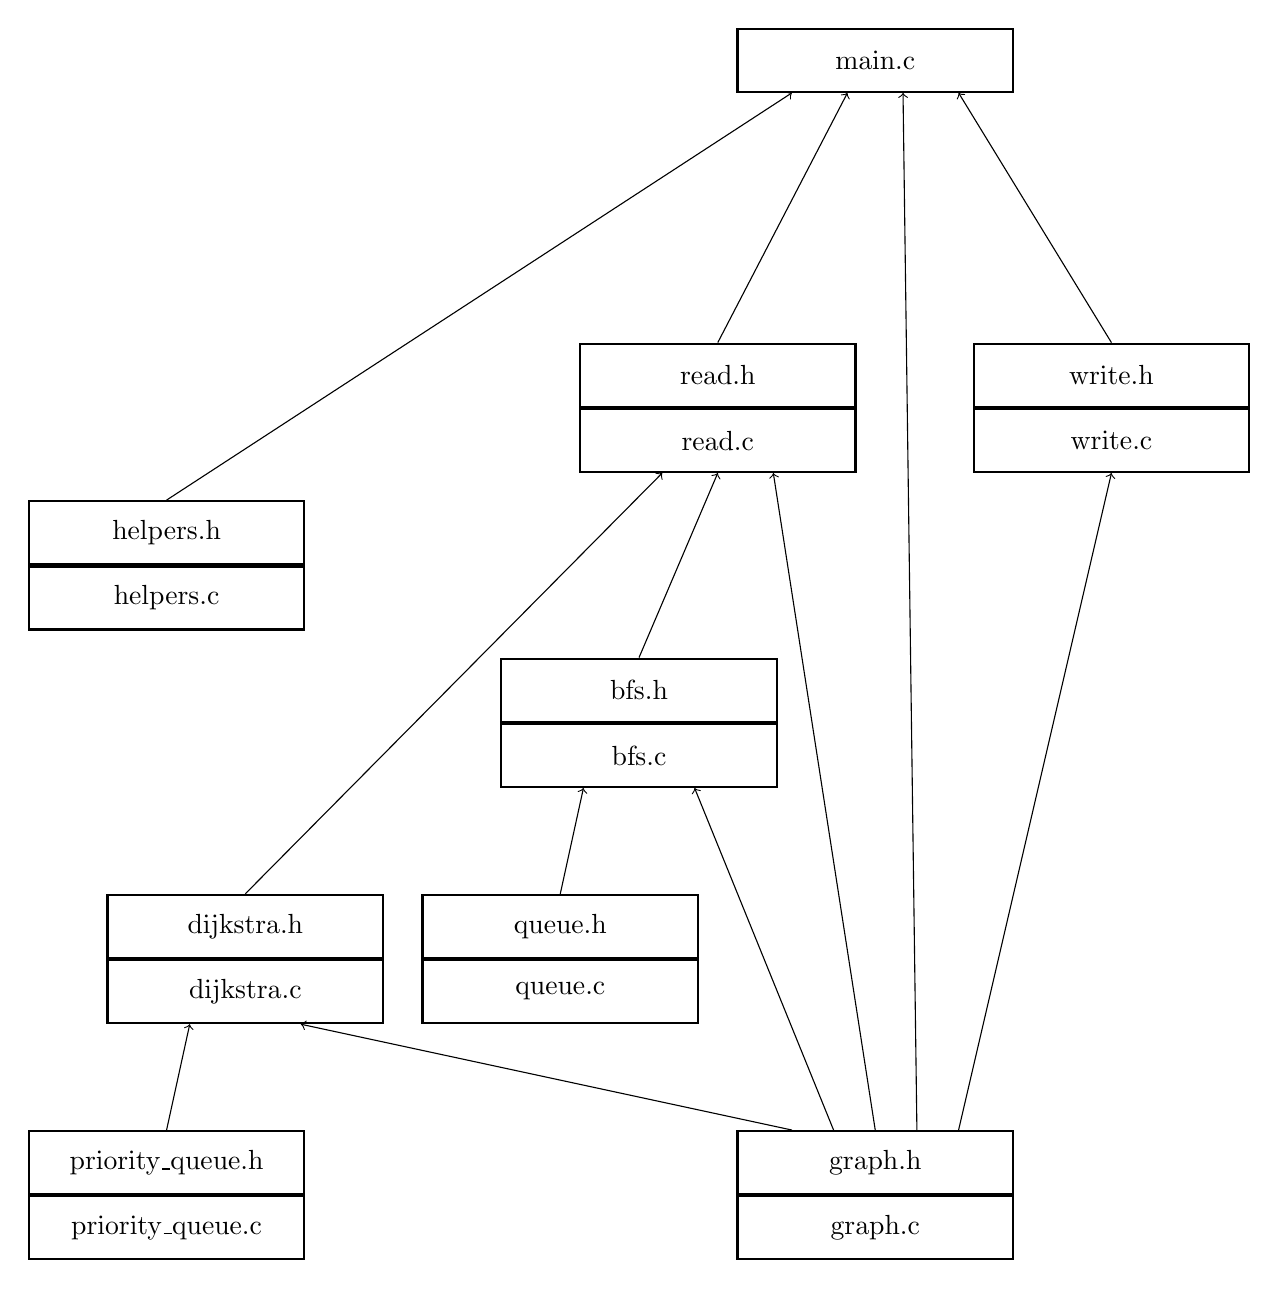
\begin{tikzpicture}
            [
                file/.style={rectangle, draw, thick, minimum width=3.5cm, minimum height=0.8cm}
            ]
            %nodes
            \node[file] at (0,0)                        (priority_queue_h)  {priority\_queue.h};
            \node[file, below=0cm of priority_queue_h]  (priority_queue_c)  {priority\_queue.c};
            \node[file] at (5,3)                        (queue_h)           {queue.h};
            \node[file, below=0cm of queue_h]           (queue_c)           {queue.c};
            \node[file] at (0,8)                        (helpers_h)         {helpers.h};
            \node[file, below=0cm of helpers_h]         (helpers_c)         {helpers.c};
            \node[file] at (9,0)                        (graph_h)           {graph.h};
            \node[file, below=0cm of graph_h]           (graph_c)           {graph.c};
            \node[file] at (1,3)                        (dijkstra_h)        {dijkstra.h};
            \node[file, below=0cm of dijkstra_h]        (dijkstra_c)        {dijkstra.c};
            \node[file] at (6,6)                        (bfs_h)             {bfs.h};
            \node[file, below=0cm of bfs_h]             (bfs_c)             {bfs.c};
            \node[file] at (7,10)                       (read_h)            {read.h};
            \node[file, below=0cm of read_h]            (read_c)            {read.c};
            \node[file] at (12,10)                      (write_h)           {write.h};
            \node[file, below=0cm of write_h]           (write_c)           {write.c};
            \node[file] at (9,14)                       (main_c)            {main.c};
            %arrows
            \draw[->] (priority_queue_h.north) -- ($(dijkstra_c.south west)!0.3!(dijkstra_c.south east)$);
            \draw[->] (queue_h.north) -- ($(bfs_c.south west)!0.3!(bfs_c.south east)$);
            \draw[->] ($(graph_h.north west)!0.2!(graph_h.north east)$) -- ($(dijkstra_c.south west)!0.7!(dijkstra_c.south east)$);
            \draw[->] ($(graph_h.north west)!0.35!(graph_h.north east)$) -- ($(bfs_c.south west)!0.7!(bfs_c.south east)$);
            \draw[->] ($(graph_h.north west)!0.5!(graph_h.north east)$) -- ($(read_c.south west)!0.7!(read_c.south east)$);
            \draw[->] ($(graph_h.north west)!0.65!(graph_h.north east)$) -- ($(main_c.south west)!0.6!(main_c.south east)$);
            \draw[->] ($(graph_h.north west)!0.8!(graph_h.north east)$) -- (write_c.south);
            \draw[->] (helpers_h.north) -- ($(main_c.south west)!0.2!(main_c.south east)$);
            \draw[->] (dijkstra_h.north) -- ($(read_c.south west)!0.3!(read_c.south east)$);
            \draw[->] (bfs_h.north) -- ($(read_c.south west)!0.5!(read_c.south east)$);
            \draw[->] (read_h.north) -- ($(main_c.south west)!0.4!(main_c.south east)$);
            \draw[->] (write_h.north) -- ($(main_c.south west)!0.8!(main_c.south east)$);
        \end{tikzpicture}
    \end{center}

    \vspace{2em}

    \noindent
    \textbf{Objaśnienie:}

    \begin{center}
        \begin {tikzpicture}
            [
                file/.style={rectangle, draw, thick, minimum width=2cm, minimum height=0.6cm}
            ]
            \node[file] at (0,0)                    (queue_h)       {queue.h};
            \node[file, below=0cm of queue_h]       (queue_c)       {queue.c};
            \node[file] at (0,2)                    (read_h)        {read.h};
            \node[file, below=0cm of read_h]        (read_c)        {read.c};
            \draw[->] (queue_h.north) -- (read_c.south);
        \end{tikzpicture}
    \end{center}

    Plik \console{queue.h} jest dołączany do pliku \console{read.c} (oraz ewentualnie do \console{read.h}). To znaczy że w pliku \console{read.c} (oraz ewentualnie w \console{read.h}) znajduje się dyrektywa \console{\#include "queue.h"}.

    

    \newpage
    \section{Plik main.c}

    Plik źródłowy (main.c) zawiera stałe \console{*\_o} i \console{help} oraz definicje funkcji:
    \begin{itemize}
        \item \console{write\_init}
        \item \console{read\_init}
        \item \console{main}
    \end{itemize}

    \subsection{Stałe \console{*\_o}}

    \console{const char* *\_o[2]} (np. \console{const char* file\_o[2]})

    \vspace{0.5em}

    Stałe te przechowują nazwy argumentów wywołania, gdzie pierwszym elementem jest długa (normalna) nazwa argumentu, a drugim nazwa skrócona.

    \subsection{Stała \console{help}}

    \console{const char* help}

    \vspace{0.5em}

    Stała ta przechowuje pomoc, zawierającą instrukcję wywołania i opisy wszystkich argumentów.

    \subsection{Funkcja \console{write\_init}}

    \console{int write\_init(int argc, char* argv[])}

    \vspace{0.5em}

    Funkcja ta sprawdza argumenty wywołania dla trybu zapisu i ich wartości, a następnie wywołuje funkcję odpowiedzialną za tryb zapisu. Funkcja zwraca wartości \console{EXIT\_SUCCESS} lub \console{EXIT\_FAILURE}.

    \subsection{Funkcja \console{read\_init}}

    \console{int read\_init(int argc, char* argv[])}

    \vspace{0.5em}

    Funkcja ta sprawdza argumenty wywołania dla trybu czytania i ich wartości, a następnie wywołuje funkcję odpowiedzialną za tryb czytania. Funkcja zwraca wartości \console{EXIT\_SUCCESS} lub \console{EXIT\_FAILURE}.

    \subsection{Funkcja \console{main}}

    \console{int main(int argc, char* argv[])}

    \vspace{0.5em}

    Funkcja ta sprawdza, który tryb został wybrany, a następnie wywołuje funkcje \console{write\_init} lub \console{read\_init} (lub wyświetla pomoc jeżeli tryb nie został wybrany). Funkcja zwraca wartości \console{EXIT\_SUCCESS} lub \console{EXIT\_FAILURE}.



    \newpage
    \section{Pliki write.c i .h}

    Plik źródłowy (write.c) zawiera stałą \console{ec\_drawing\_weight} oraz definicje funkcji:
    \begin{itemize}
        \item \console{gen\_graph}
        \item \console{write}*
    \end{itemize}

    Plik nagłówkowy (write.h) zawiera deklaracje zaznaczonych funkcji z pliku źródłowego (*).

    \subsection{Stała \console{ec\_drawing\_weight}}

    \console{const int ec\_drawing\_weight[5]}

    \vspace{0.5em}
    
    Stała ta przechowuje informację o wagach losowania dla poszczególnych liczb krawędzi. Na przykład wartości \console{\{1,2,3,4,5\}} oznaczają że wraz z liczbą krawędzi rośnie szansa na wylosowanie danej liczby krawędzi, gdyż tablica z której losowana będzie liczba krawędzi będzie wyglądać tak: \console{\{0,1,1,2,2,2,3,3,3,3,4,4,4,4,4\}}.

    \subsection{Funkcja \console{gen\_graph}}

    \console{graph gen\_graph(int width, int height, double edge\_weight\_min, double edge\_weight\_max, int edge\_count\_min, int edge\_count\_max, int seed)}

    \vspace{0.5em}
    
    Funkcja ta odpowiada za wygenerowanie grafu o szerokości (ilości kolumn) \console{width}, wysokości (ilości wierzy) \console{height}, gdzie każdy wierzchołek będzie miał maksymalnie \console{edge\_count\_max} i (w miarę możliwości) minimalnie \console{edge\_count\_min} krawędzi \footnote{liczba krawędzi jest losowana; patrz "Stała \console{ec\_drawing\_weight}"}, z których każda będzie miała wagę mieszczącą się w przedziale od \console{edge\_weight\_min} do \console{edge\_weight\_max} włącznie. Funkcja zwraca graf.

    \subsection{Funkcja \console{write}}

    \console{int write(FILE* file, int width, int height, double edge\_weight\_min, double edge\_weight\_max, int edge\_count\_min, int edge\_count\_max, int seed)}

    \vspace{0.5em}
    
    Funkcja ta wywołuje funkcję \console{gen\_graph} (przekazując jej jednocześnie wszystkie swoje parametry poza \console{file}), a następnie zapisuje uzyskany graf do pliku \console{file}. Funkcja zwraca wartości \console{EXIT\_SUCCESS} lub \console{EXIT\_FAILURE} (funkcja nie przewiduje wystąpienia błędu, więc w praktyce jest to tylko \console{EXIT\_SUCCESS}).



    \newpage
    \section{Pliki read.c i .h}

    Plik źródłowy (read.c) zawiera definicje funkcji:
    \begin{itemize}
        \item \console{path\_fill}
        \item \console{path\_display}
        \item \console{bfs\_init}
        \item \console{dijkstra\_init}
        \item \console{read\_graph}
        \item \console{read}*
    \end{itemize}

    Plik nagłówkowy (read.h) zawiera deklaracje zaznaczonych funkcji z pliku źródłowego (*).

    \subsection{Funkcja \console{path\_fill}}

    \console{int path\_fill(d\_result result, int *nv, int from, int to)}

    \vspace{0.5em}
    
    Funkcja ta odpowiada za wypełnienie tablicy \console{nv} numerami wierzchołków, które tworzą ścieżkę od \console{from} do \console{to}, na podstawie tablicy poprzedników wygenerowanej przez algorytm Dijkstry i przechowywanej w strukturze \console{result}. Funkcja zwraca ilość dodanych wierzchołków do tablicy.

    \subsection{Funkcja \console{path\_display}}

    \console{void path\_display(int *nv, int l)}

    \vspace{0.5em}
    
    Funkcja ta odpowiada za wyświetlenie ścieżki pomiędzy dwoma wierzchołkami przechowywanej w tablicy \console{nv} znając jej długość \console{l}.

    \subsection{Funkcja \console{bfs\_init}}

    \console{void bfs\_init(graph g)}

    \vspace{0.5em}

    Funkcja ta odpowiada za wywołanie algorytmu BFS i wyświetlenie komunikatu o spójności grafu \console{g}.
    \subsection{Funkcja \console{dijkstra\_init}}

    \console{void dijkstra\_init(graph g, int vertex\_a, int vertex\_b)}

    \vspace{0.5em}
    
    Funkcja ta odpowiada za wywołanie algorytmu Dijkstry i wyświetlenie najkrótszej ścieżki pomiędzy wierzchołkami \console{vertex\_a} i \console{vertex\_b} lub najkrótszych ścieżek pomiędzy wierzchołkiem \console{vertex\_a} i pozostałymi wierzchołkami grafu \console{g}.

    \subsection{Funkcja \console{read\_graph}}

    \console{graph read\_graph(FILE *f)}

    \vspace{0.5em}
    
    Funkcja ta odpowiada za odczytanie grafu z pliku \console{f}, tworzenie struktury grafu i uzupełnienie jej przeczytanymi wierzchołkami i wagami z pliku. Funkcja zwraca stworzoną strukturę grafu.

    \subsection{Funkcja \console{read}}

    \console{int read(FILE *file, int connectivity, int vertex\_a, int vertex\_b)}

    \vspace{0.5em}
    
    Funkcja odpowiada za zarządzanie trybem read. Przyjmuje wskaźnik na plik (bądź stdin), z którego ma być czytany graf, a także czy ma być sprawdzona jego spójność (\console{connectivity} przyjmuje wartość 1/0) oraz numery wierzchołków, między którymi ma być wyznaczona ścieżka (gdy \console{vertex\_b} jest równy -1, wyznaczana jest ścieżka pomiędzy \console{vertex\_a} i wszystkimi wierzchołkami).



    \newpage
    \section{Pliki dijkstra.c i .h}
    Plik źródłowy (dijkstra.c) zawiera definicje funkcji:
    \begin{itemize}
        \item \console{result\_init}*
        \item \console{result\_free}*
        \item \console{dijkstra}*
    \end{itemize}

    Plik nagłówkowy (dijkstra.h) poza deklaracjami zaznaczonych funkcji z pliku źródłowego (*) zawiera także deklarację struktury wyniku generowanego przez algorytm Dijkstry (\console{d\_result}).

    \subsection{Struktura \console{d\_result}}

    \begin{multiconsole}
        typedef struct r

        \{

        \hspace{1em} double *d;

        \hspace{1em} int *p;

        \} *d\_result;
    \end{multiconsole}

    \vspace{0.5em}

    Struktura przechowuje dwie tablice: \console{d} - zawierającą całkowitą wagę dojścia do danego wierzchołka z wierzchołka początkowego oraz \console{p} – zawierającą numery poprzedników.

    \subsection{Funkcja \console{result\_init}}

    \console{d\_result result\_init(int n, int vertex\_a, int *visited)}
    
    \vspace{0.5em}

    Funkcja ta odpowiada za zainicjalizowanie struktury typu \console{d\_result} i wypełnienie jej tablic w taki sposób jaki wymaga tego algorytm Dijkstry (tablica \console{d} wypełniona nieskończonościami oprócz elementu o indeksie wierzchołka początkowego; tablica \console{p} wypełniona wartościami -1). Funkcja zwraca utworzoną strukturę.

    \subsection{Funkcja \console{result\_free}}

    \console{void result\_free(d\_result result)}

    \vspace{0.5em}
    
    Funkcja ta odpowiada za zwolnienie pamięci zarezerwowanej dla struktury \console{result}.

    \subsection{Funkcja \console{dijkstra}}

    \console{d\_result dijkstra(graph graph, int vertex\_a)}

    \vspace{0.5em}
    
    Funkcja ta jest implementacją algorytmu Dijkstry wykorzystującego kolejkę priorytetową do uzupełnienia tablic struktury typu \console{d\_result}. Funkcja jako argument przyjmuje \console{vertex\_a} (numer wierzchołka startowego) oraz \console{vertex\_b}. Jeżeli szukana jest ścieżka wyłącznie do jednego wierzchołka, algorytm przerywa działanie w momencie dojścia do wierzchołka docelowego (\console{vertex\_b}). Funkcja zwraca utworzoną strukturę.



    \newpage
    \section{Pliki bfs.c i .h}

    Plik źródłowy (bfs.c) zawiera definicje funkcji:
    \begin{itemize}
        \item \console{bfs}*
    \end{itemize}

    Plik nagłówkowy (bfs.h) zawiera deklaracje zaznaczonych funkcji z pliku źródłowego (*).

    \subsection{Funkcja \console{bfs}}

    \console{int* bfs(graph graph, int vertex)}

    \vspace{0.5em}
    
    Funkcja ta jest implementacją algorytmu BFS (Breadth-first search) w uproszczonej wersji. Sprawdza czy w grafie \console{graph} od wierzchołka \console{vertex} istnieją ścieżki do wszystkich pozostałych wierzchołków. Funkcja zwraca tablicę liczb 0/1 (prawda/fałsz) o długości [ilość wierzchołków grafu], w której index oznacza numer wierzchołka a wartość wynik sprawdzenia dla wierzchołka o danym indeksie.



    \newpage
    \section{Pliki graph.c i .h}

    Plik źródłowy (graph.c) zawiera definicje funkcji:
    \begin{itemize}
        \item \console{graph\_init}*
        \item \console{graph\_free}*
        \item \console{edge\_list\_add}*
        \item \console{edge\_list\_contains\_vertex}*
        \item \console{edge\_list\_length}*
    \end{itemize}

    Plik nagłówkowy (graph.h) poza deklaracjami zaznaczonych funkcji z pliku źródłowego (*) zawiera także deklarację struktury grafu w formie listy sąsiedztwa (\console{graph}) oraz deklarację struktury listy wierzchołków (\console{edge\_list}).

    \subsection{Struktura \console{graph}}
    \begin{multiconsole}
        typedef struct g

        \{

        \hspace{1em} int width;

        \hspace{1em} int height;

        \hspace{1em} edge\_list **list;

        \} *graph;
    \end{multiconsole}

    \vspace{0.5em}

    Struktura przechowuje szerokość grafu (liczba kolumn) (\console{width}), wysokość grafu (liczba wierszy) (\console{height}) oraz tablicę list połączonych wierzchołków dla każdego wierzchołka (lista sąsiedztwa) (\console{list}).

    \subsection{Struktura \console{edge\_list}}

    \begin{multiconsole}
        typedef struct e

        \{

        \hspace{1em} int vertex;

        \hspace{1em} double weight;

        \hspace{1em} struct e *next;

        \} edge\_list;
    \end{multiconsole}
    
    \vspace{0.5em}

    Struktura przechowuje numer połączonego wierzchołka (\console{vertex}), wagę krawędzi (\console{weight}) oraz wskaźnik na następny element (\console{next}) (lista jednokierunkowa).

    \subsection{Funkcja \console{graph\_init}}

    \console{graph graph\_init(int w, int h)}

    \vspace{0.5em}
    
    Funkcja ta odpowiada za zainicjalizowanie grafu o szerokości (ilości kolumn) \console{w} i wysokości (ilości wierszy) \console{h}. Funkcja zwraca graf.

    \subsection{Funkcja \console{graph\_free}}

    \console{void graph\_free(graph g)}

    \vspace{0.5em}
    
    Funkcja ta odpowiada za zwolnienie pamięci zarezerwowanej dla grafu \console{g}.

    \subsection{Funkcja \console{edge\_list\_add}}

    \console{edge\_list* edge\_list\_add(edge\_list *l, int v, double wt)}
    
    \vspace{0.5em}

    Funkcja ta odpowiada za dodanie na koniec listy połączonych wierzchołów \console{l} nowego wierzchołka o numerze \console{v} i wadze krawędzi \console{wt}. Funkcja zwraca wskaźnik na listę połączonych wierzchołków.

    \subsection{Funkcja \console{edge\_list\_contains\_vertex}}

    \console{int edge\_list\_contains\_vertex(edge\_list* l, int v)}
    
    \vspace{0.5em}

    Funkcja ta odpowiada za sprawdzenie czy na liście połączonych wierzchołków \console{l} znajduje się wierzchołek o numerze \console{v}. Funkcja zwraca wartości 1/0 (prawda/fałsz).

    \subsection{Funkcja \console{edge\_list\_length}}

    \console{int edge\_list\_length(edge\_list* l)}
    
    Funkcja ta odpowiada za sprawdzenie długości listy połączonych wierzchołków \console{l}. Funkcja zwraca długość listy.



    \newpage
    \section{Pliki queue.c i .h}

    Plik źródłowy (queue.c) zawiera definicje funkcji:
    \begin{itemize}
        \item \console{queue\_enqueue}*
        \item \console{queue\_dequeue}*
    \end{itemize}

    Plik nagłówkowy (queue.h) poza deklaracjami zaznaczonych funkcji z pliku źródłowego (*) zawiera także deklarację struktury kolejki FIFO (First in, first out) (\console{queue}).

    \subsection{Struktura \console{queue}}

    \begin{multiconsole}
        typedef struct q

        \{

        \hspace{1em} int value;

        \hspace{1em} struct q* next;

        \} queue;
    \end{multiconsole}
    
    \vspace{0.5em}
    
    Struktura przechowuje wartość pojedyńczego elementu (\console{value}) oraz wskaźnik na następny element (\console{next}) (lista jednokierunkowa).

    \subsection{Funkcja \console{queue\_enqueue}}

    \console{void queue\_enqueue(queue** q, int value)}
    
    \vspace{0.5em}

    Funkcja ta odpowiada za dodanie na początku kolejki \console{q} (listy) nowego elementu o wartości \console{value}.

    \subsection{Funkcja \console{queue\_enqueue}}

    \console{int queue\_dequeue(queue** q)}

    \vspace{0.5em}
    
    Funkcja ta odpowiada za pobranie wartości elementu z końca kolejki \console{q} (listy), usunięcie ostatniego elementu z kolejki, a następnie zwrócenie pobranej wartości.



    \newpage
    \section{Pliki priority\_queue.c i .h}

    Plik źródłowy (priority\_queue.c) zawiera definicje funkcji:
    \begin{itemize}
        \item \console{pq\_init}*
        \item \console{pq\_is\_empty}*
        \item \console{heap\_up}*
        \item \console{pq\_push}*
        \item \console{heap\_down}
        \item \console{pq\_pop}*
        \item \console{pq\_free}*
    \end{itemize}

    Plik nagłówkowy (priority\_queue.h) poza deklaracjami zaznaczonych funkcji z pliku źródłowego (*) zawiera także deklarację struktury kolejki priorytetowej (\console{pq}).

    \subsection{Struktura \console{pq}}

    \begin{multiconsole}
        typedef struct p

        \{

        \hspace{1em} int *q;

        \hspace{1em} int *pn;

        \hspace{1em} int n;

        \hspace{1em} int size;

        \} *pq;
    \end{multiconsole}
    
    \vspace{0.5em}
    
    Struktura przechowuje tablicę numerów wszystkich wierzchołków (\console{q}), gdzie priorytetem jest najmniejsza odległość od wierzchołka źródłowego. Tablica \console{pn} przechowuje pozycję i-tego wierzchołka w kolejce, \console{n} jest liczbą pozostałych wierzchołków, a \console{size} maksymalnym rozmiarem kolejki równym liczbie wszystkich wierzchołków w grafie.

    \subsection{Funkcja \console{pq\_init}}

    \console{pq pq\_init(int size)}
    
    \vspace{0.5em}

    Funkcja ta odpowiada za alokowanie miejsca na strukturę \console{pq} i jej pola. Funkcja zwraca tą strukturę.

    \subsection{Funkcja \console{pq\_is\_empty}}

    \console{int pq\_is\_empty(pq p\_queue)}

    \vspace{0.5em}
    
    Funkcja sprawdza czy kolejka jest pusta. Funkcja zwraca wartości 1/0 (prawda/fałsz).

    \subsection{Funkcja \console{heap\_up}}

    \console{void heap\_up(pq p\_queue, double *d, int from)}

    \vspace{0.5em}
    
    Funkcja ta odpowiada za implementację przesiewania kopca w górę. Wykorzystywana do tego jest tablica \console{d}, która przechowuje odległości wierzchołków od wierzchołka źródłowego, które są priorytetem. Funkcja przyjmuje także argument \console{from}, który jest indeksem kopca, od którego należy rozpocząć przesiewanie (przydatne w algorytmie Dijkstry).

    \subsection{Funkcja \console{pq\_push}}

    \console{int pq\_push(pq p\_queue, double *d, int v)}

    \vspace{0.5em}
    
    Funkcja ta odpowiada za dodanie do kolejki priorytetowej numeru wierzchołka \console{v} i wywołanie funkcji \console{heap\_up}. Funkcja ta jest używana tylko podczas testów i nie wykorzystuje jej algorytm Dijkstry.

    \subsection{Funkcja \console{heap\_down}}

    \console{static void heap\_down(pq p\_queue, double *d)}

    \vspace{0.5em}
    
    Funkcja ta odpowiada za implementację przesiewania kopca w dół. Wykorzystywana do tego jest tablica \console{d}, która przechowuje odległości wierzchołków od wierzchołka źródłowego, które są priorytetem.

    \subsection{Funkcja \console{pq\_pop}}

    \console{int pq\_pop(pq p\_queue, double *d)}

    \vspace{0.5em}
    
    Funkcja ta odpowiada za usunięcie z kolejki priorytetowej wierzchołka znajdującego się w korzeniu i wywołanie funkcji \console{heap\_down}. Funkcja zwraca numer zdjętego wierzchołka.

    \subsection{Funkcja \console{pq\_free}}

    \console{void pq\_free(pq p\_queue)}

    \vspace{0.5em}
    
    Funkcja ta odpowiada za zwolnienie pamięci zarezerwowanej dla kolejki \console{p\_queue}



    \newpage
    \section{Pliki helpers.c i .h}

    Plik źródłowy (helpers.c) zawiera definicje funkcji:
    \begin{itemize}
        \item \console{str\_arr\_get\_index}*
        \item \console{str\_is\_int}*
        \item \console{str\_is\_double}*
    \end{itemize}

    Plik nagłówkowy (helpers.h) zawiera deklaracje zaznaczonych funkcji z pliku źródłowego (*).

    \subsection{Funkcja \console{str\_arr\_get\_index}}

    \console{int str\_arr\_get\_index(char* element, const char* array[], int length)}

    \vspace{0.5em}
    
    Funkcja ta odpowiada za znalezienie w tablicy napisów \console{array} o długości \console{length} konkretnego napisu \console{element}. Funkcja zwraca indeks tego napisu w tablicy.

    \subsection{Funkcja \console{str\_is\_int}}

    \console{int str\_is\_int(char* string)}

    \vspace{0.5em}
    
    Funkcja ta odpowiada za sprawdzenie czy napis \console{string} jest liczbą całkowitą (tzn. napis zawiera tylko cyfry i ewentualnie znak minus na początku). Funkcja zwraca wartości 1/0 (prawda/fałsz).

    \subsection{Funkcja \console{str\_is\_double}}

    \console{int str\_is\_double(char* string)}
    
    \vspace{0.5em}

    Funkcja ta odpowiada za sprawdzenie czy napis \console{string} jest liczbą rzeczywistą (tzn. napis zawiera tylko cyfry oraz ewentualnie jedną kropkę i znak minus na początku). Funkcja zwraca wartości 1/0 (prawda/fałsz).



    \newpage
    \section{Plik makefile}

    Plik makefile przechowuje instrukcje kompilacji programu oraz instrukcję czyszczenia folderu (\console{clean}) i instrukcję testu (\console{test}).

    \subsection{Kompilacja (\console{make})}

    Instrukcja kompilacji składa się z czterech etapów:
    \begin{enumerate}
        \item wygenerowania pliku zawierającego zależności (\console{cc -MM [pliki źródłowe] $>$ [plik zaw. zależności]})
        \item wczytania go (\console{-include [plik zaw. zależności]})
        \item skompilowania programu (\console{cc -o gridgraph [pliki .o]})
        \item czyszczenia pokompilacyjnego (\console{rm [pliki .o] [plik zaw. zależności]})
    \end{enumerate}

    \subsection{Czyszczenie (\console{make clean})}

    Instrukcja czyszczenia usuwa pliki (wywoływana jest komenda \console{rm [pliki]}):
    \begin{itemize}
        \item plik programu
        \item pliki .o
        \item plik zawierający zależności
    \end{itemize}

    \subsection{Test (\console{make test})}

    Instrukcja testu w pierwszej kolejności wywołuje instrukcję kompilacji, a następnie usuwa folder zawierający wyniki testów (domyślnie: "./test\_results"), tworzy go i na koniec wywołuje kolejne testy opisane w rozdziale "Testy".



    \chapter{Testy}
    


    \newpage
    \section{Generowanie małego grafu 6x6 z domyślnymi parametrami}

    Test polega na wygenerowaniu grafu o rozmiarach 6 na 6 z domyślnymi pozostałymi parametrami i zapisaniu go do pliku "test1" w folderze zawierającym wyniki testów. 
    
    Plik powinien zawierać 27 linii. W pierwszej powinna być zapisana długość i wysokość grafu (\console{5 5}), a w następnych 25 lista sąsiedztwa, gdzie dla każdego wierzchołka powinno być od 0 do 4 krawędzi, z których każda powinna mieć wagę mieszczącą się w przedziale od 0 do 1. Ostatnia linia powinna być pusta.

    \vspace{2em}

    \textbf{Wywoływane komendy:}

    \vspace{1em}

    \begin{multiconsole}
        ./gridgraph -w -xw 5 -xh 5 -f [folder zaw. wyn. testów]/test1
    \end{multiconsole}

    \vspace{2em}

    \textbf{Przykładowy wynik testu zakończonego powodzeniem:}

    \vspace{1em}

    Plik "test1":

    \begin{multiconsole}
        5 5

        \hspace{2em}5 :0.141989  1 :0.588184 

        \hspace{2em}0 :0.588184  2 :0.374213  6 :0.753903 

        \hspace{2em}1 :0.374213  7 :0.012313  3 :0.115006 

        [... pominięto 19 linii ...]

        \hspace{2em}21 :0.775892  23 :0.844664 

        \hspace{2em}18 :0.961897  22 :0.844664  24 :0.048494 

        \hspace{2em}19 :0.151187  23 :0.048494
    \end{multiconsole}


    \newpage
    \section{Generowanie dużego grafu 1000x1000 z domyślnymi parametrami}

    Test polega na wygenerowaniu grafu o rozmiarach 1000 na 1000 z domyślnymi pozostałymi parametrami i zapisaniu go do pliku "test2" w folderze zawierającym wyniki testów. 
    
    Plik powinien zawierać 1000002 linie. W pierwszej powinna być zapisana długość i wysokość grafu (\console{1000 1000}), a w następnych 1000000 lista sąsiedztwa, gdzie dla każdego wierzchołka powinno być od 0 do 4 krawędzi, z których każda powinna mieć wagę mieszczącą się w przedziale od 0 do 1. Ostatnia linia powinna być pusta.

    \vspace{2em}

    \textbf{Wywoływane komendy:}

    \vspace{1em}

    \begin{multiconsole}
        ./gridgraph -w -xw 1000 -xh 1000 -f [folder zaw. wyn. testów]/test2
    \end{multiconsole}

    \vspace{2em}

    \textbf{Przykładowy wynik testu zakończonego powodzeniem:}

    \vspace{1em}

    Plik "test2":

    \begin{multiconsole}
        1000 1000

        \hspace{2em}1000 :0.337479  1 :0.003876 

        \hspace{2em}0 :0.003876  2 :0.098184  1001 :0.338146 

        \hspace{2em}1 :0.098184  1002 :0.693836  3 :0.853243 

        [... pominięto 999994 linie ...]

        \hspace{2em}999996 :0.167250  999998 :0.136315 

        \hspace{2em}998998 :0.988869  999997 :0.136315  999999 :0.805686 

        \hspace{2em}998999 :0.235517  999998 :0.805686 
    \end{multiconsole}
    


    \newpage
    \section{Generowanie grafu 50x50 ze stałym ziarnem generatora liczb losowych}

    Test polega na wygenerowaniu dwóch grafów o rozmiarach 50 na 50, ziarnem generatora liczb losowych równym 0 i z domyślnymi pozostałymi parametrami i zapisaniu ich odpowiednio do plików "test3" i "test4", a następnie sprawdzeniu ich identyczności oraz identyczności z plikiem zawierającym oczekiwany graf. 
    
    Oba pliki powinny zawierać 2502 linie każdy. W pierwszej powinna być zapisana długość i wysokość grafu (\console{50 50}), a w następnych 2500 lista sąsiedztwa, gdzie dla każdego wierzchołka powinno być od 0 do 4 krawędzi, z których każda powinna mieć wagę mieszczącą się w przedziale od 0 do 1. Ostatnia linia powinna być pusta. 
    
    Oba pliki powinny być identyczne. Co więcej pliki powinny być identyczne jak te co w poprzednim wywołaniu testu. Identyczność plików jest sprawdzana programem \console{cmp} (najpierw identyczność obu plików, a następnie identyczność z plikiem "expected\_test3" zawierający spodziewany dla tego testu graf). Po każdym wywołaniu programu \console{cmp} wypisywany jest kod zakończenia. Wszystkie powinny być równe 0.

    \vspace{2em}

    \textbf{Wywoływane komendy:}

    \vspace{1em}

    \begin{multiconsole}
        ./gridgraph -w -xw 50 -xh 50 -s 0 -f [folder zaw. wyn. testów]/test3

        ./gridgraph -w -xw 50 -xh 50 -s 0 -f [folder zaw. wyn. testów]/test4

        cmp [folder zaw. wyn. testów]/test3 [folder zaw. wyn. testów]/test4

        echo \$?

        cmp [folder zaw. wyn. testów]/test3 ./Tests/expected\_test3

        echo \$?
    \end{multiconsole}

    \vspace{2em}

    \textbf{Przykładowy wynik testu zakończonego powodzeniem:}

    \vspace{1em}

    Pliki "test3" i "test4" \footnote{Cała zawartość w pliku "Tests/expected\_text3"} \footnote{Pliki powinny być identyczne jak przedstawiony przykład}:

    \begin{multiconsole}
        50 50

        \hspace{2em}1 :0.743163  50 :0.092576 

        \hspace{2em}0 :0.743163  51 :0.482107 

        \hspace{2em}3 :0.329285  52 :0.311602 

        [... pominięto 2494 linie ...]

        \hspace{2em}2447 :0.383774  2496 :0.584013 

        \hspace{2em}2448 :0.722728  2499 :0.981057 

        \hspace{2em}2449 :0.113450  2498 :0.981057  
    \end{multiconsole}


    \newpage
    \section{Generowanie grafu 50x50 na pewno niespójnego (granica liczby krawędzi od 0 do 1) i sprawdzenie spójności}

    Test polega na wygenerowaniu grafu który na pewno będzie niespójny, o rozmiarach 50 na 50, granicą liczby krawędzi od 0 do 1 i z domyślnymi pozostałymi parametrami i zapisaniu go do pliku "test5" w folderze zawierającym wyniki testów, a następnie na sprawdzeniu jego spójności, zapisaniu wyniku sprawdzenia w pliku "test6" i porównaniu wyniku sprawdzenia z oczekiwanym.
    
    Plik "test5" powinien zawierać 2502 linie. W pierwszej powinna być zapisana długość i wysokość grafu (\console{50 50}), a w następnych 2500 lista sąsiedztwa, gdzie dla każdego wierzchołka powinno być od 0 do 1 krawędzi, z których każda powinna mieć wagę mieszczącą się w przedziale od 0 do 1. Ostatnia linia powinna być pusta. Plik "test6" powinien zawierać 3 linie, z których w pierwszej powinien być wypisany wynik testu spójności, a dwie pozostałe powinny być puste.
    
    Identyczność pliku zawierającego wynik sprawdzenia ("test6") z plikiem zawierającym oczekiwany wynik sprawdzenia ("expected\_test6") jest sprawdzana programem \console{cmp}. Po wywołaniu programu \console{cmp} wypisywany jest kod zakończenia, ktry powinien by równy 0.

    \vspace{2em}

    \textbf{Wywoływane komendy:}

    \vspace{1em}

    \begin{multiconsole}
        ./gridgraph -w -xw 50 -xh 50 -Cmax 1 -f [folder zaw. wyn. testów]/test5

        ./gridgraph -r -c -f [folder zaw. wyn. testów]/test5 > [folder zaw. wyn. testów]/test6

        cmp [folder zaw. wyn. testów]/test6 ../Tests/expected\_test6

        echo \$?
    \end{multiconsole}

    \vspace{2em}

    \textbf{Przykładowy wynik testu zakończonego powodzeniem:}

    \vspace{1em}

    Plik "test5":

    \begin{multiconsole}
        50 50

        \hspace{2em}1 :0.938031

        \hspace{2em}0 :0.938031 

        \hspace{2em}52 :0.782637

        [... pominięto 2494 linie ...]

        \hspace{2em}

        \hspace{2em}

        \hspace{2em}2449 :0.331057   
    \end{multiconsole}

    \vspace{1em}

    Plik "test6" \footnote{Plik powinien być identyczny jak przedstawiony przykład}:

    \begin{multiconsole}
        Connectivity: disconnected
    \end{multiconsole}


    \newpage
    \section{Generowanie grafu 50x50 na pewno spójnego (granica liczby krawędzi od 4 do 4) i sprawdzenie spójności}

    Test polega na wygenerowaniu grafu który na pewno będzie spójny, o rozmiarach 50 na 50, granicą liczby krawędzi od 4 do 4 i z domyślnymi pozostałymi parametrami i zapisaniu go do pliku "test7" w folderze zawierającym wyniki testów, a następnie na sprawdzeniu jego spójności, zapisaniu wyniku sprawdzenia w pliku "test8" i porównaniu wyniku sprawdzenia z oczekiwanym.
    
    Plik "test7" powinien zawierać 2502 linie. W pierwszej powinna być zapisana długość i wysokość grafu (\console{50 50}), a w następnych 2500 lista sąsiedztwa, gdzie każdy wierzchołek powinien mieć 4 krawędzie\footnote{Jeżeli to możliwe}, z których każda powinna mieć wagę mieszczącą się w przedziale od 0 do 1. Ostatnia linia powinna być pusta. Plik "test8" powinien zawierać 3 linie, z których w pierwszej powinien być wypisany wynik testu spójności, a dwie pozostałe powinny być puste.
    
    Identyczność pliku zawierającego wynik sprawdzenia ("test8") z plikiem zawierającym oczekiwany wynik sprawdzenia ("expected\_test8") jest sprawdzana programem \console{cmp}. Po wywołaniu programu \console{cmp} wypisywany jest kod zakończenia, ktry powinien by równy 0.

    \vspace{2em}

    \textbf{Wywoływane komendy:}

    \vspace{1em}

    \begin{multiconsole}
        ./gridgraph -w -xw 50 -xh 50 -Cmin 4 -f [folder zaw. wyn. testów]/test7

        ./gridgraph -r -c -f [folder zaw. wyn. testów]/test7 > [folder zaw. wyn. testów]/test8

        cmp [folder zaw. wyn. testów]/test8 ../Tests/expected\_test8

        echo \$?
    \end{multiconsole}

    \vspace{2em}

    \textbf{Przykładowy wynik testu zakończonego powodzeniem:}

    \vspace{1em}

    Plik "test7":

    \begin{multiconsole}
        50 50

        \hspace{2em}1 :0.719183  50 :0.750156 

        \hspace{2em}0 :0.719183  51 :0.448654  2 :0.136224

        \hspace{2em}1 :0.136224  3 :0.087748  52 :0.258144

        [... pominięto 2494 linie ...]

        \hspace{2em}2447 :0.796042  2496 :0.107598  2498 :0.043867

        \hspace{2em}2448 :0.404981  2497 :0.043867  2499 :0.831039

        \hspace{2em}2449 :0.912295  2498 :0.831039
    \end{multiconsole}

    \vspace{1em}

    Plik "test8" \footnote{Plik powinien być identyczny jak przedstawiony przykład}:

    \begin{multiconsole}
        Connectivity: connected
    \end{multiconsole}


    \newpage
    \section{Generowanie grafu 50x50 o wagach krawędzi od 0.3 do 0.7}

    Test polega na wygenerowaniu grafu o rozmiarach 50 na 50, o wagach krawędzi mieszczących się w granicach od 0.3 do 0.7 i z domyślnymi pozostałymi parametrami i zapisaniu go do pliku "test9" w folderze zawierającym wyniki testów. 
    
    Plik powinien zawierać 2502 linie. W pierwszej powinna być zapisana długość i wysokość grafu (\console{50 50}), a w następnych 2500 lista sąsiedztwa, gdzie dla każdego wierzchołka powinno być od 0 do 4 krawędzi, z których każda powinna mieć wagę mieszczącą się w przedziale od 0.3 do 0.7. Ostatnia linia powinna być pusta.

    \vspace{2em}

    \textbf{Wywoływane komendy:}

    \vspace{1em}

    \begin{multiconsole}
        ./gridgraph -w -xw 50 -xh 50 -Wmin 0.3 -Wmax 0.7 -f [folder zaw. wyn. testów]/test9
    \end{multiconsole}

    \vspace{2em}

    \textbf{Przykładowy wynik testu zakończonego powodzeniem:}

    \vspace{1em}

    Plik "test9":

    \begin{multiconsole}
        50 50

        \hspace{2em}1 :0.587673  50 :0.600063

        \hspace{2em}0 :0.587673  51 :0.479462  2 :0.354490 

        \hspace{2em}1 :0.354490  3 :0.335099 

        [... pominięto 2494 linie ...]

        \hspace{2em}2447 :0.401067  2496 :0.697442  2498 :0.340867 

        \hspace{2em}2448 :0.496822  2497 :0.340867 

        \hspace{2em}2449 :0.425698
    \end{multiconsole}


    \newpage
    \section{Generowanie grafu 100x100, o stałym ziarnie generatora liczb losowych, granicy liczby krawędzi od 1 do 3 i wagach krawędzi od 0.4 do 0.9 oraz sprawdzenie najkrótszych ścieżek od wierzchołka 0 do pozostałych wierzchołków}

    Test polega na wygenerowaniu grafu o rozmiarach 100 na 100, ziarnem generatora liczb losowych równym 0, granicą liczby krawędzi od 1 do 3 i wagach krawędzi od 0.4 do 0.9 i zapisaniu go do pliku "test10" w folderze zawierającym wyniki testów, a następnie sprawdzeniu jego z plikiem zawierającym oczekiwany graf. W ramach testu sprawdzane są także najkrótsze ścieżki od wierzchołka 0 do pozostałych wierzchołków. Wynik sprawdzenia zapisywany jest w pliku "test11", a następnie porównanywany z oczekiwanym.

    Plik "test10" powinien zawierać 10002 linie. W pierwszej powinna być zapisana długość i wysokość grafu (\console{100 100}), a w następnych 10000 lista sąsiedztwa, gdzie dla każdego wierzchołka powinno być od 1 \footnote{Jeżeli to możliwe} do 3 krawędzi, z których każda powinna mieć wagę mieszczącą się w przedziale od 0.4 do 0.9. Ostatnia linia powinna być pusta. Plik "test11" powinien zawierać 10003 linie, z których w dwóch pierwszych znajduje się nagłówek testu, a w następnych 10000, ścieżki do określonych wierzchołków (wraz z wagami). Ostatnia linia powinna być pusta.

    Identyczność plików jest sprawdzana programem \console{cmp} (najpierw identyczność pliku zawierającego graf ("test10") z plikiem "expected\_test10", a następnie identyczność pliku zawierającego wynik sprawdzenia ("test11") z plikiem "expected\_test11"). Po każdym wywołaniu programu \console{cmp} wypisywany jest kod zakończenia. Wszystkie powinny być równe 0.

    \vspace{2em}

    \textbf{Wywoływane komendy:}

    \vspace{1em}

    \begin{multiconsole}
        ./gridgraph -w -xw 100 -xh 100 -Cmin 1 -Cmax 3 -Wmin 0.4 -Wmax 0.9 -s 0 -f [folder zaw. wyn. testów]/test10

        cmp [folder zaw. wyn. testów]/test10 ../Tests/expected\_test10

        echo \$?

        ./gridgraph -r -sA 0 -f [folder zaw. wyn. testów]/test10 > [folder zaw. wyn. testów]/test11

        cmp [folder zaw. wyn. testów]/test11 ../Tests/expected\_test11

        echo \$?
    \end{multiconsole}

    \vspace{2em}

    \textbf{Przykładowy wynik testu zakończonego powodzeniem:}

    \vspace{1em}

    Plik "test10" \footnote{Cała zawartość w pliku "Tests/expected\_text10"} \footnote{Plik powinnien być identyczny jak przedstawiony przykład}:

    \begin{multiconsole}
        100 100

        \hspace{2em}100 :0.828420

        \hspace{2em}2 :0.577575  101 :0.736913 

        \hspace{2em}1 :0.577575  3 :0.787888  102 :0.684638 

        [... pominięto 9994 linie ...]

        \hspace{2em}9996 :0.871117  9998 :0.714386

        \hspace{2em}9898 :0.608558  9997 :0.714386 

        \hspace{2em}9899 :0.818561 

    \end{multiconsole}

    \vspace{1em}

    Plik "test11" \footnote{Cała zawartość w pliku "Tests/expected\_text11"} \footnote{Plik powinnien być identyczny jak przedstawiony przykład}:

    \begin{multiconsole}
        Shortest paths from 0 to all vertices and their weights:

        

        Path to 0 (weight): 0 (0) 

        Path to 1 (weight): 0 - 100 - 200 - 201 - 202 - 102 - 2 - 1 (5.07255)

        Path to 2 (weight): 0 - 100 - 200 - 201 - 202 - 102 - 2 (4.49497)

        [... pominięto 9994 linie ...]

        Path to 9997 (weight): 0 - 100 - [... pominięto 1788 znaków ...] - 9998 - 9997 (166.437)

        Path to 9998 (weight): 0 - 100 - [... pominięto 1781 znaków ...] - 9898 - 9998 (165.863)

        Path to 9999 (weight): 0 - 100 - [... pominięto 1788 znaków ...] - 9899 - 9999 (166.64)
    \end{multiconsole}


    \newpage
    \section{Sprawdzenie poprawności działania kolejki priorytetowej}

    Test polega na posortowaniu 1000 liczb wylosowanych z zakresu od 0 do 1 wykorzystując przy tym kolejkę priorytetową. Wyniki sortowania zapisywane są do pliku „test12” w folderze zawierającym wyniki testów.
    
    Plik powinien zawierać 1003 linie. W pierwszej linii powinna być zapisana informacja o sortowaniu kopcowym. Następne 1000 linii to liczby, które powinny być uporządkowane rosnąco. W 1002 linii powinna pojawić się informacja o tym czy kolejka priorytetowa działa poprawnie (program testujący sprawdza również czy liczby na pewno są posortowane). Ostatnia linia powinna być pusta.

    W ramach testu na początku kompilowany jest także program testujący, który na koniec jest usuwany.

    \vspace{2em}

    \textbf{Wywoływane komendy:}

    \vspace{1em}

    \begin{multiconsole}
        cc -o pq\_test priority\_queue.c ../Tests/priority\_queue\_test.c

        ./pq\_test 1000 [folder zaw. wyn. testów]/test12

        rm pq\_test
    \end{multiconsole}

    \vspace{2em}

    \textbf{Przykładowy wynik testu zakończonego powodzeniem:}

    Plik "test12":

    \begin{multiconsole}
        Heap sort:

        0.000368076

        0.000576437

        0.00139771

        [… pominięto 994 linie … ]

        0.998762

        0.99949

        0.999512

        Priority queue works properly.
    \end{multiconsole}
\end{document}